\section{Exo-Planet Examples} \label{sec:app}
In this section, we perform the proposed AAIS method to deal with
two real RV data set.

\subsection{Star HD73526}
This data set contains 18 data components, and were claimed to
support an orbit of $190.5\pm3.0$ days \citep{tinney2003four}.
\cite{gregory2005bayesian} did a Bayesian re-analysis on this data
set using a parallel tempering MCMC algorithm, and reported three
possible orbits, with periods $127.88_{-0.09}^{+0.37}$,
$190.4_{-2.1}^{+1.8}$ and $376.2_{-4.3}^{+1.4}$ days, respectively.
\cite{gregory2005bayesian} also discussed the possibility of having
an additional planet, and reported that the Bayes factor is less
than 1 when comparing $\mathcal{M}_2$ with the $\mathcal{M}_1$.

We use the proposed AAIS algorithm to deal with $\mathcal{M}_0$,
$\mathcal{M}_1$ and $\mathcal{M}_2$, respectively. The marginal
likelihood estimation result is summarized in Table
\ref{marginal_likelihood_data1}. These estimates are reliable
indicated by their corresponding \ESS$/N$. The resulting Bayes
factors are shown in Table \ref{Bayes_factor_data1}. As indicated by
the result, this data set support the one-planet hypothesis, which
coincides the conclusions made by
\cite{tinney2003four,gregory2005bayesian}.

\begin{table}
\begin{tabular}{c|c|c}
 & Marginal Likelihood & \ESS$/N$\\
\hline $\mathcal{M}_0$ & $5.9013\times10^{-50}\pm5.1325\times10^{-52}$ & 0.9320\\
\hline $\mathcal{M}_1$ & $4.4886\times10^{-41}\pm3.2093\times10^{-42}$ & 0.5698\\
\hline $\mathcal{M}_2$ & $1.5511\times10^{-42}\pm3.2878\times10^{-43}$ & 0.3458\\
\hline
\end{tabular}
\caption{HD73526 \cite{tinney2003four} Data Case. The calculated
marginal likelihoods}\label{marginal_likelihood_data1}
\end{table}

\begin{table}
\begin{tabular}{c|c}
 \BF$\{\mathcal{M}_1:\mathcal{M}_0\}$ & \BF$\{\mathcal{M}_2:\mathcal{M}_1\}$\\
\hline $7.606\times10^8$& 0.03456\\
\hline
\end{tabular}
\caption{HD73526 \citep{tinney2003four} Data Case. The calculated
Bayes Factors}\label{Bayes_factor_data1}
\end{table}

Specifically for $\mathcal{M}_1$, we show the posterior samples
(equally weighted by resampling) in Fig. \ref{fig:scatter_1p_data1}.
 We obtain two modes in $P$, that are $P_1=190.1_{-1.5}^{+2.2}$ and
$P_2=375.5_{-2.5}^{+2.0}$, respectively.

\begin{figure}[!htb]
\centerline{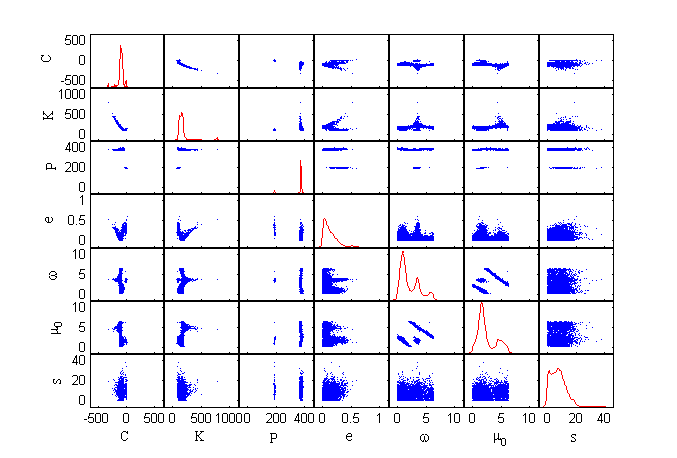
\includegraphics[width=4in,height=3.2in]{Fig/scatter_1p_data1.png}}
\caption{HD73526 \cite{tinney2003four} Data Case. Scatter plot of
the posterior samples of
$\mathcal{M}_1$}\label{fig:scatter_1p_data1}
\end{figure}

\subsection{Star HD73526}
This data set contains 30 RV data components and was claimed to have
two planets \citep{tinney20062}.

We calculate the marginal likelihoods using the proposed AAIS
algorithm, and the result is shown in Table
\ref{marginal_likelihood_data2}. Indicated by the criterion
\ESS$/N$, we deem that the result is reliable. The resulting Bayes
factors can be seen in Table \ref{Bayes_factor_data2}. So our result
supports the argument in \cite{tinney20062}$-$there are two planets
underlying this data set.

\begin{table}
\begin{tabular}{c|c|c}
 & Marginal Likelihood & \ESS$/N$\\
\hline $\mathcal{M}_0$ & $8.9566\times10^{-77}\pm1.0852\times10^{-78}$ & 0.9510\\
\hline $\mathcal{M}_1$ & $5.8519\times10^{-70}\pm1.7077\times10^{-71}$ & 0.6545\\
\hline $\mathcal{M}_2$ & $4.8122\times10^{-65}\pm1.4284\times10^{-66}$ & 0.2034 \\
\hline
\end{tabular}
\caption{HD73526 \citep{tinney20062} Data Case. The calculated
marginal likelihoods}\label{marginal_likelihood_data2}
\end{table}

\begin{table}
\begin{tabular}{c|c}
 \BF$\{\mathcal{M}_1:\mathcal{M}_0\}$ & \BF$\{\mathcal{M}_2:\mathcal{M}_1\}$\\
\hline $6.534\times10^6$& $8.233\times10^4$\\
\hline
\end{tabular}
\caption{HD73526 \citep{tinney20062} Data Case. The calculated
Bayes Factors}\label{Bayes_factor_data2}
\end{table}

The posterior samples (equally weighted by resampling) corresponding
to $\mathcal{M}_1$ is shown in Fig.\ref{fig:scatter_1p_data2}, and
the algorithm again captures two modes in $P$, that are
$P_1=193.1162_{-3.7}^{+2.1}$ and $P_2=374.8732_{-5.8}^{+6.9}$.

When dealing with $\mathcal{M}_2$, we still restrict the period of
the first planet to be smaller than that of the second planet.
Fig.\ref{fig:scatter_2p_data2} shows the posterior samples of
$\mathcal{M}_2$. Given these posterior samples, we get the periods
of the two planets, that are $P_1=187.9379_{-0.8}^{+2.1}$ and
$P_2=377.3030_{-4.5}^{+5.2}$, respectively.
\begin{figure}[!htb]
\centerline{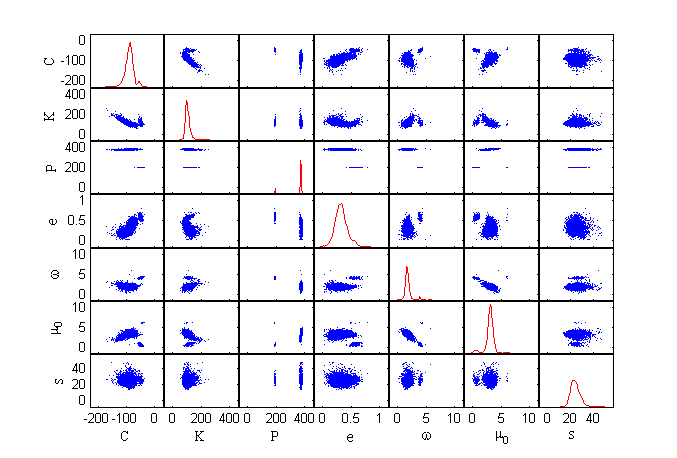
\includegraphics[width=4in,height=3.2in]{Fig/scatter_1p_data2.png}}
\caption{HD73526 \citep{tinney20062} Data Case. Scatter plot of the
posterior samples of $\mathcal{M}_1$}\label{fig:scatter_1p_data2}
\end{figure}

\begin{figure}[!htb]
\begin{tabular}{c}
\centerline{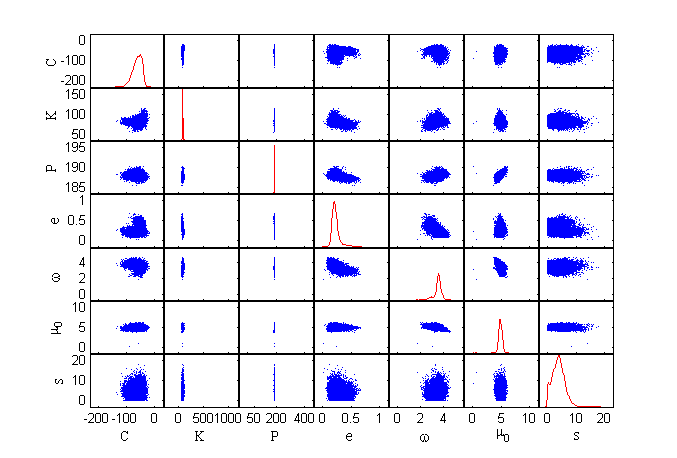
\includegraphics[width=4in,height=3.2in]{Fig/scatter1_2p_data2.png}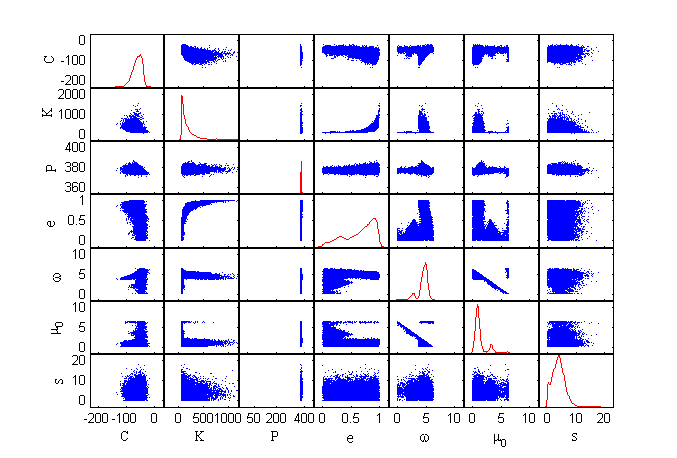
\includegraphics[width=4in,height=3.2in]{Fig/scatter2_2p_data2.png}}\\
\end{tabular}
\caption{HD73526 \cite{tinney20062} Data Case. Scatter plot of the
posterior samples of $\mathcal{M}_2$. Left: Scatter plot of the
posterior samples of the first planet parameter; Right: Scatter plot
of the posterior samples of the second planet parameter}
\label{fig:scatter_2p_data2}
\end{figure}


Given samples from the posterior, we can easily get the minimum mean
squared estimate (MMSE) of the RV at any given time, and then plot
the RV curve. In Fig.\ref{fig:rv_comparison_data2}, we plot the
estimated RV curves on basis of $\mathcal{M}_0$, $\mathcal{M}_1$ and
$\mathcal{M}_2$, respectively, meanwhile the real RV observations
are depicted there for reference. As in shown, the RV estimation
yielded by $\mathcal{M}_2$ fits the real data best.

\begin{figure}[!htb]
\centerline{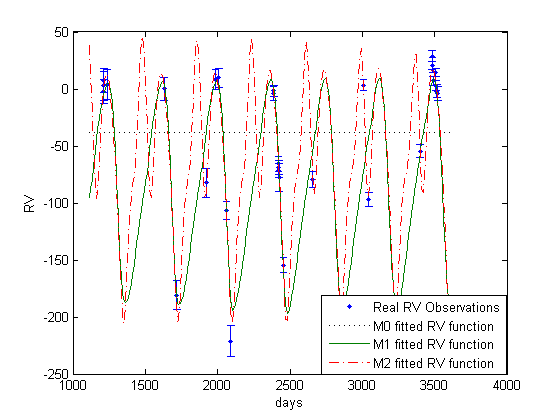
\includegraphics[width=4in,height=3.2in]{Fig/rv_comparison_data2.png}}
\caption{Measured velocities (filled circles) vs. time for HD73526
\cite{tinney20062}. Error bars only includes internal uncertainties.
The curves are MMSE estimates of the RV yielded by $\mathcal{M}_0$,
$\mathcal{M}_1$ and $\mathcal{M}_2$,
respectively}\label{fig:rv_comparison_data2}
\end{figure}

\subsection{The HD217107 Data Case}
Star HD217107 was claimed to have two planets \citep{vogt2005five}.

We analyze the observed RV data for HD217107 using our AAIS method,
the calculated marginal likelihoods are shown in Table
\ref{marginal_likelihood_HD217107}, each corresponding to a
sufficiently big value of \ESS$/N$. The resulting Bayes factors can
be seen in Table \ref{Bayes_factor_HD217107}. It's shown that
$\mathcal{M}_2$ beats both $\mathcal{M}_0$ and $\mathcal{M}_1$.

\begin{table}
\begin{tabular}{c|c|c}
 & Marginal Likelihood & \ESS$/N$\\
\hline $\mathcal{M}_0$ & $3.6492\times10^{-168}\pm7.0150\times10^{-169}$ & 0.9644\\
\hline $\mathcal{M}_1$ & $3.7389\times10^{-141}\pm0.6077\times10^{-142}$ & 0.6448\\
\hline $\mathcal{M}_2$ & $3.0897\times10^{-108}\pm1.0011\times10^{-109}$ & 0.4119 \\
\hline
\end{tabular}
\caption{HD217107 \citep{vogt2005five} Data Case. The calculated
marginal likelihoods}\label{marginal_likelihood_HD217107}
\end{table}

\begin{table}
\begin{tabular}{c|c}
 \BF$\{\mathcal{M}_1:\mathcal{M}_0\}$ & \BF$\{\mathcal{M}_2:\mathcal{M}_1\}$\\
\hline $1.025\times10^{27}$& $8.264\times10^{32}$\\
\hline
\end{tabular}
\caption{HD217107 \citep{vogt2005five} Data Case. The calculated
Bayes Factors}\label{Bayes_factor_HD217107}
\end{table}

\subsection{The HD37124 Data Case}
Star HD37124 was claimed to have three planets \citep{vogt2005five}.

We analyze the associated RV data set using our AAIS method, the
marginal likelihoods calculated by our AAIS algorithm are shown in
Table \ref{marginal_likelihood_37124}. Indicated by the criterion
\ESS$/N$, the results are reliable. The resulting Bayes factors can
be seen in Table \ref{Bayes_factor_37124}, which support the
conclusion of \cite{tinney20062}, i.e. this data set supports the
three-planet hypothesis.

\begin{table}
\begin{tabular}{c|c|c}
 & Marginal Likelihood & \ESS$/N$\\
\hline $\mathcal{M}_0$ & $2.0889\times10^{-110}\pm2.1857\times10^{-112}$ & 0.9427\\
\hline $\mathcal{M}_1$ & $1.0717\times10^{-106}\pm1.3077\times10^{-107}$ & 0.1737\\
\hline $\mathcal{M}_2$ & $1.9830\times10^{-97}\pm1.1451\times10^{-98}$ & 0.1798 \\
\hline $\mathcal{M}_3$ & $2.9228\times10^{-84}\pm1.2563\times10^{-85}$ & 0.1305 \\
\hline
\end{tabular}
\caption{HD37124 \citep{vogt2005five} Data Case. The calculated
marginal likelihoods}\label{marginal_likelihood_37124}
\end{table}

\begin{table}
\begin{tabular}{c|c|c}
\BF$\{\mathcal{M}_1:\mathcal{M}_0\}$ &\BF$\{\mathcal{M}_2:\mathcal{M}_1\}$ & \BF$\{\mathcal{M}_3:\mathcal{M}_2\}$\\
\hline $5.13\times10^3$ & $1.850\times10^9$ & $1.474\times10^{13}$\\
\hline
\end{tabular}
\caption{HD37124 \citep{vogt2005five} Data Case. The calculated
Bayes Factors}\label{Bayes_factor_37124}
\end{table}

In Fig.\ref{fig:hd37124_fit}, we plot the estimated RV curves on
basis of $\mathcal{M}_1$, $\mathcal{M}_2$ and $\mathcal{M}_3$,
respectively, where the real RV observations is also depicted for
reference. As is shown, the RV estimation yielded by $\mathcal{M}_3$
fits the real data best.



\begin{figure}[!htb]
\begin{tabular}{c}
\centerline{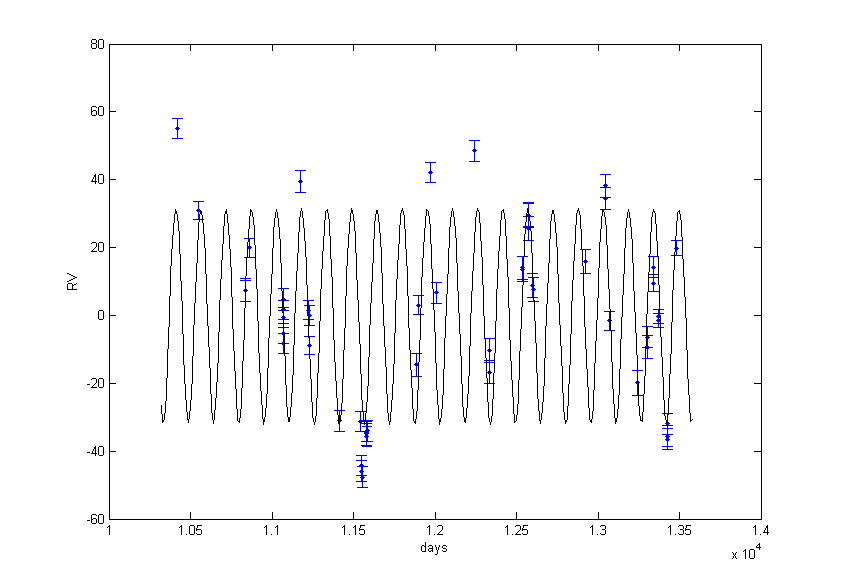
\includegraphics[width=4in,height=3.2in]{Fig/hd37124_1p_fit.png}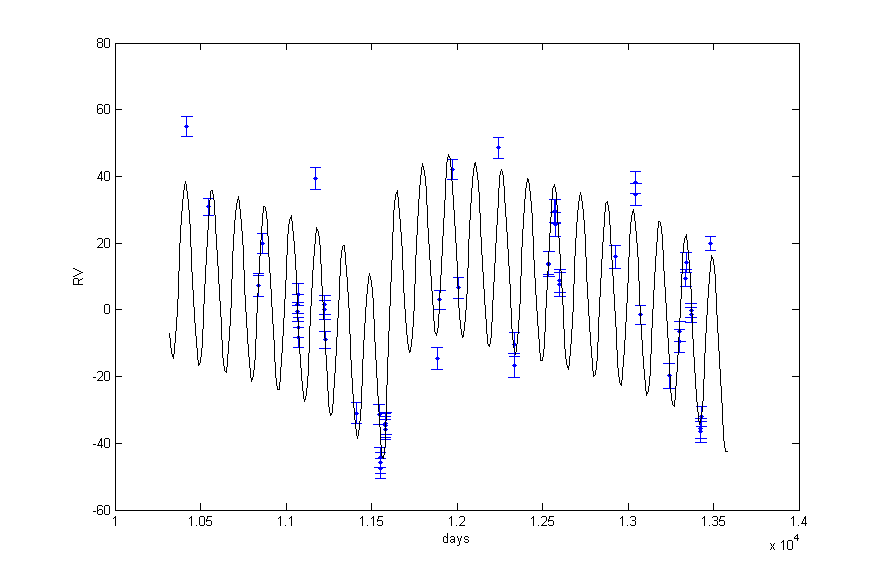
\includegraphics[width=4in,height=3.2in]{Fig/hd37124_2p_fit.png}}\\
\centerline{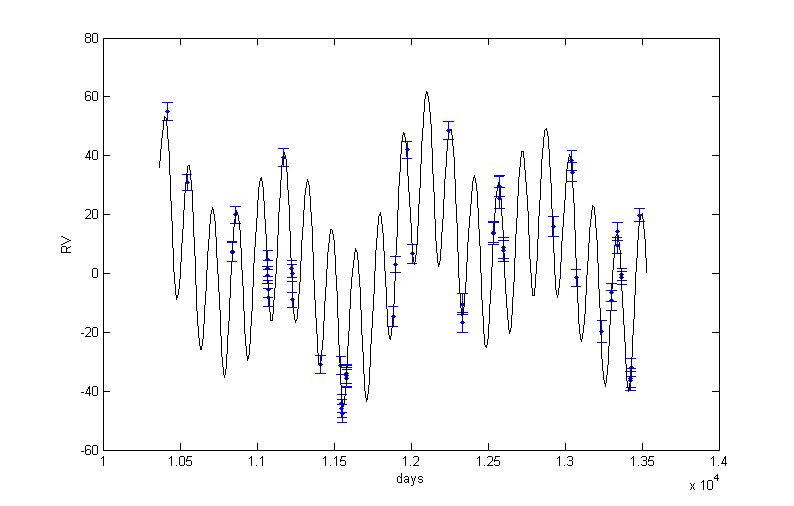
\includegraphics[width=4in,height=3.2in]{Fig/hd37124_3p_fit.png}}
\end{tabular}
\caption{Measured velocities (filled circles) vs. time for HD37124
\cite{tinney20062}. Error bars only includes internal uncertainties.
The MMSE estimates of the RV curves yielded by using
$\mathcal{M}_1$, $\mathcal{M}_2$ and $\mathcal{M}_3$ are shown in
the top left, top right and the bottom panels, respectively.}
\label{fig:hd37124_fit}
\end{figure}

\subsection{The 47 Ursae Majoris (47 UMa) Data Case}
This 47 UMa data recently was analyzed in
\cite{gregory2010bayesian}.

We analyze the associated RV data set using our AAIS method, the
marginal likelihoods calculated by our AAIS algorithm are shown in
Table \ref{marginal_likelihood_uma47}. We obtain reliable estimates
for $\mathcal{M}_0$, $\mathcal{M}_1$ and $\mathcal{M}_2$, while the
estimate for $\mathcal{M}_3$ is unreliable, the \ESS$/N$ is 0.0089,
which is not big enough. Indicated by the criterion \ESS$/N$, the
results are reliable. So we argue that this data set supports
$\mathcal{M}_2$ more than $\mathcal{M}_0$ and $\mathcal{M}_1$, but
we are not sure about the relative strength between $\mathcal{M}_2$
and $\mathcal{M}_3$. \cite{gregory2010bayesian} concluded that this
data set has three planets, however, gave an much ambiguous estimate
for the third planet's period.

\begin{table}
\begin{tabular}{c|c|c}
 & Marginal Likelihood & \ESS$/N$\\
\hline $\mathcal{M}_0$ & $2.0198\times10^{-1004}\pm9.2572\times10^{-1006}$ & 0.1002\\
\hline $\mathcal{M}_1$ & $3.4400\times10^{-896}\pm3.10\times10^{-897}$ & 0.5643\\
\hline $\mathcal{M}_2$ & $1.3500\times10^{-816}\pm1.77\times10^{-817}$ & 0.3324 \\
\hline $\mathcal{M}_3$ & $2.8970\times10^{-825}\pm9.1623\times10^{-825}$ & 0.0089 \\
\hline
\end{tabular}
\caption{uma47 \citep{gregory2010bayesian} Data Case. The
calculated marginal likelihoods}\label{marginal_likelihood_uma47}
\end{table}

\begin{table}
\begin{tabular}{c|c|c}
 \BF$\{\mathcal{M}_1:\mathcal{M}_0\}$ & \BF$\{\mathcal{M}_2:\mathcal{M}_1\}$ & \BF$\{\mathcal{M}_3:\mathcal{M}_2\}$\\
\hline $1.703\times10^{108}$ & $3.924\times10^{79}$ & $ ?$\\
\hline
\end{tabular}
\caption{uma47 \citep{gregory2010bayesian} Data Case. The
calculated Bayes Factors}\label{Bayes_factor_uma47}
\end{table}

In Fig.\ref{fig:uma47_fit}, we plot the estimated RV curves on basis
of $\mathcal{M}_1$, $\mathcal{M}_2$ respectively, and again the real
RV observations are depicted there for reference. As is shown, the
RV estimation yielded by $\mathcal{M}_2$ fits better.

\begin{figure}[!htb]
\begin{tabular}{c}
\centerline{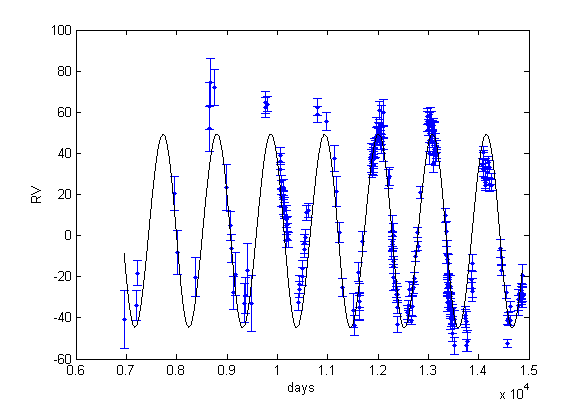
\includegraphics[width=4in,height=3.2in]{Fig/uma47_1p_fit.png}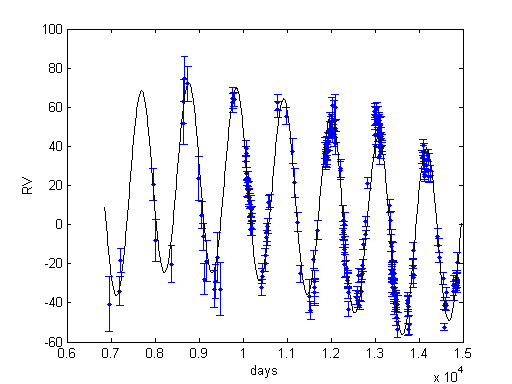
\includegraphics[width=4in,height=3.2in]{Fig/uma47_2p_fit.png}}
\end{tabular}
\caption{Measured velocities (filled circles) vs. time for the 47
Ursae Majoris (47 UMa) \citep{gregory2010bayesian}. Error bars only
includes internal uncertainties. The MMSE estimates of the RV curves
yielded by using $\mathcal{M}_1$ and $\mathcal{M}_2$ are shown in
the left and the right panels, respectively.} \label{fig:uma47_fit}
\end{figure}

